\chapter{NNQS Exploration}\label{nnqsresults}
This chapter explores the performance of the NNQS solver with various architectures and training schedules. All experiments in this section were run on a subset of the entire dataset with problem sizes of $10,25,50,75,200,250$ and $10$ randomly generated problems\footnote{random seed is chosen to be from $0-9$} for each problem type and size. 

%The problem evaluation metrics are also calculated by considering the solutions from the different types of NNQS to draw a clearer comparison between architectures and training schemes.

\section{Architectures and Training Schedules}
We will utilise the Restricted Boltzmann Machine (RBM) and the Multilayer Perceptron (MLP) as the underlying architecture for NNQS. For a given input problem with $n$ variables, the RBM model will have $n$ visible nodes and $5n$ hidden nodes, while the MLP will have $n$ input nodes, $1$ hidden layer of size $5n$ and $1$ positive real output node. The RBM uses the sigmoid function, while the MLP uses the ReLU activation function for the hidden layer and a sigmoid function in the output layer. We use Gibbs sampling for the RBM and Metropolis sampling for the MLP which are introduced in \autoref{samplingmethods}.

We will also compare three training schedules for the NNQS solver---progressive, direct, and continuous. The progressive training algorithm follows \autoref{alg:progressiveagain} and has been utilised in previous experiments. In progressive training, the normalised anneal fraction $s$ is incremented by $0.1$, and the NNQS is trained until convergence for up to $100$ epochs. In direct training, described in \autoref{alg:direct}, $s$ is held constant at $1$ for all $1000$ epochs. In continuous training, described in \autoref{alg:continuous}, $s$ is gradually increased every epoch. All schedules use at most $1000$ epochs.

\begin{algorithm}
    \begin{algorithmic}
    \For {$s \in [0.1, 1.0]$ step $0.1$}
    \State Set $H(s) \leftarrow A(s)\hat{H}_0 + B(s)\hat{H}_c$;
    \State Train NNQS on $H(s)$ until convergence or until epoch limit of $100$ is reached;
    \EndFor
    \end{algorithmic}
    \caption{NNQS Progressive Schedule}
    \label{alg:progressiveagain}
\end{algorithm}

\begin{algorithm}
    \begin{algorithmic}
    \State Set $H \leftarrow A(1)\hat{H}_0 + B(1)\hat{H}_c$;
    \State Train NNQS on $H$ until convergence or until epoch limit of $1000$ is reached;
    \end{algorithmic}
    \caption{NNQS Direct Schedule}
    \label{alg:direct}
\end{algorithm}

\begin{algorithm}
    \begin{algorithmic}
    \For {$s \in [0.001, 1.0]$ step $0.001$}
    \State Set $H(s) \leftarrow A(s)\hat{H}_0 + B(s)\hat{H}_c$;
    \State Train NNQS on $H(s)$ for $1$ epoch;
    \EndFor
    \end{algorithmic}
    \caption{NNQS Continuous Schedule}
    \label{alg:continuous}
\end{algorithm}

Direct training is a baseline for training a neural network with the cost function as the problem Hamiltonian for the entire training period. Progressive training most closely resembles the quantum annealing process, where the system is kept at the ground state by training until convergence after each increment of $s$. Continuous training slowly increments $s$ but does not train until convergence and is most similar to diabatic quantum annealing, where the system is allowed to "escape" to excited states during the annealing.

\section{Results and Discussion}
We present the performance metrics for each dataset, accompanied by error bars representing the unbiased standard error of the mean. Graphs with problem sizes on the x-axis are plotted with a log scale. The performance by dataset and problem size is shown in \autoref{appendix:nnqssizegraph}.

\subsection{NAE3SAT}
For the NAE3SAT dataset, the RBM with continuous training (red) performs the best for both average normalised energy and success probability when averaged across all problem sizes, shown in \autoref{nnqs-nae3sat-average}. The RBM with progressive training (brown), and the MLP with continuous training (blue) also perform well.

\begin{figure}[!htb]
    \centering
    \subfloat[Normalised energy]{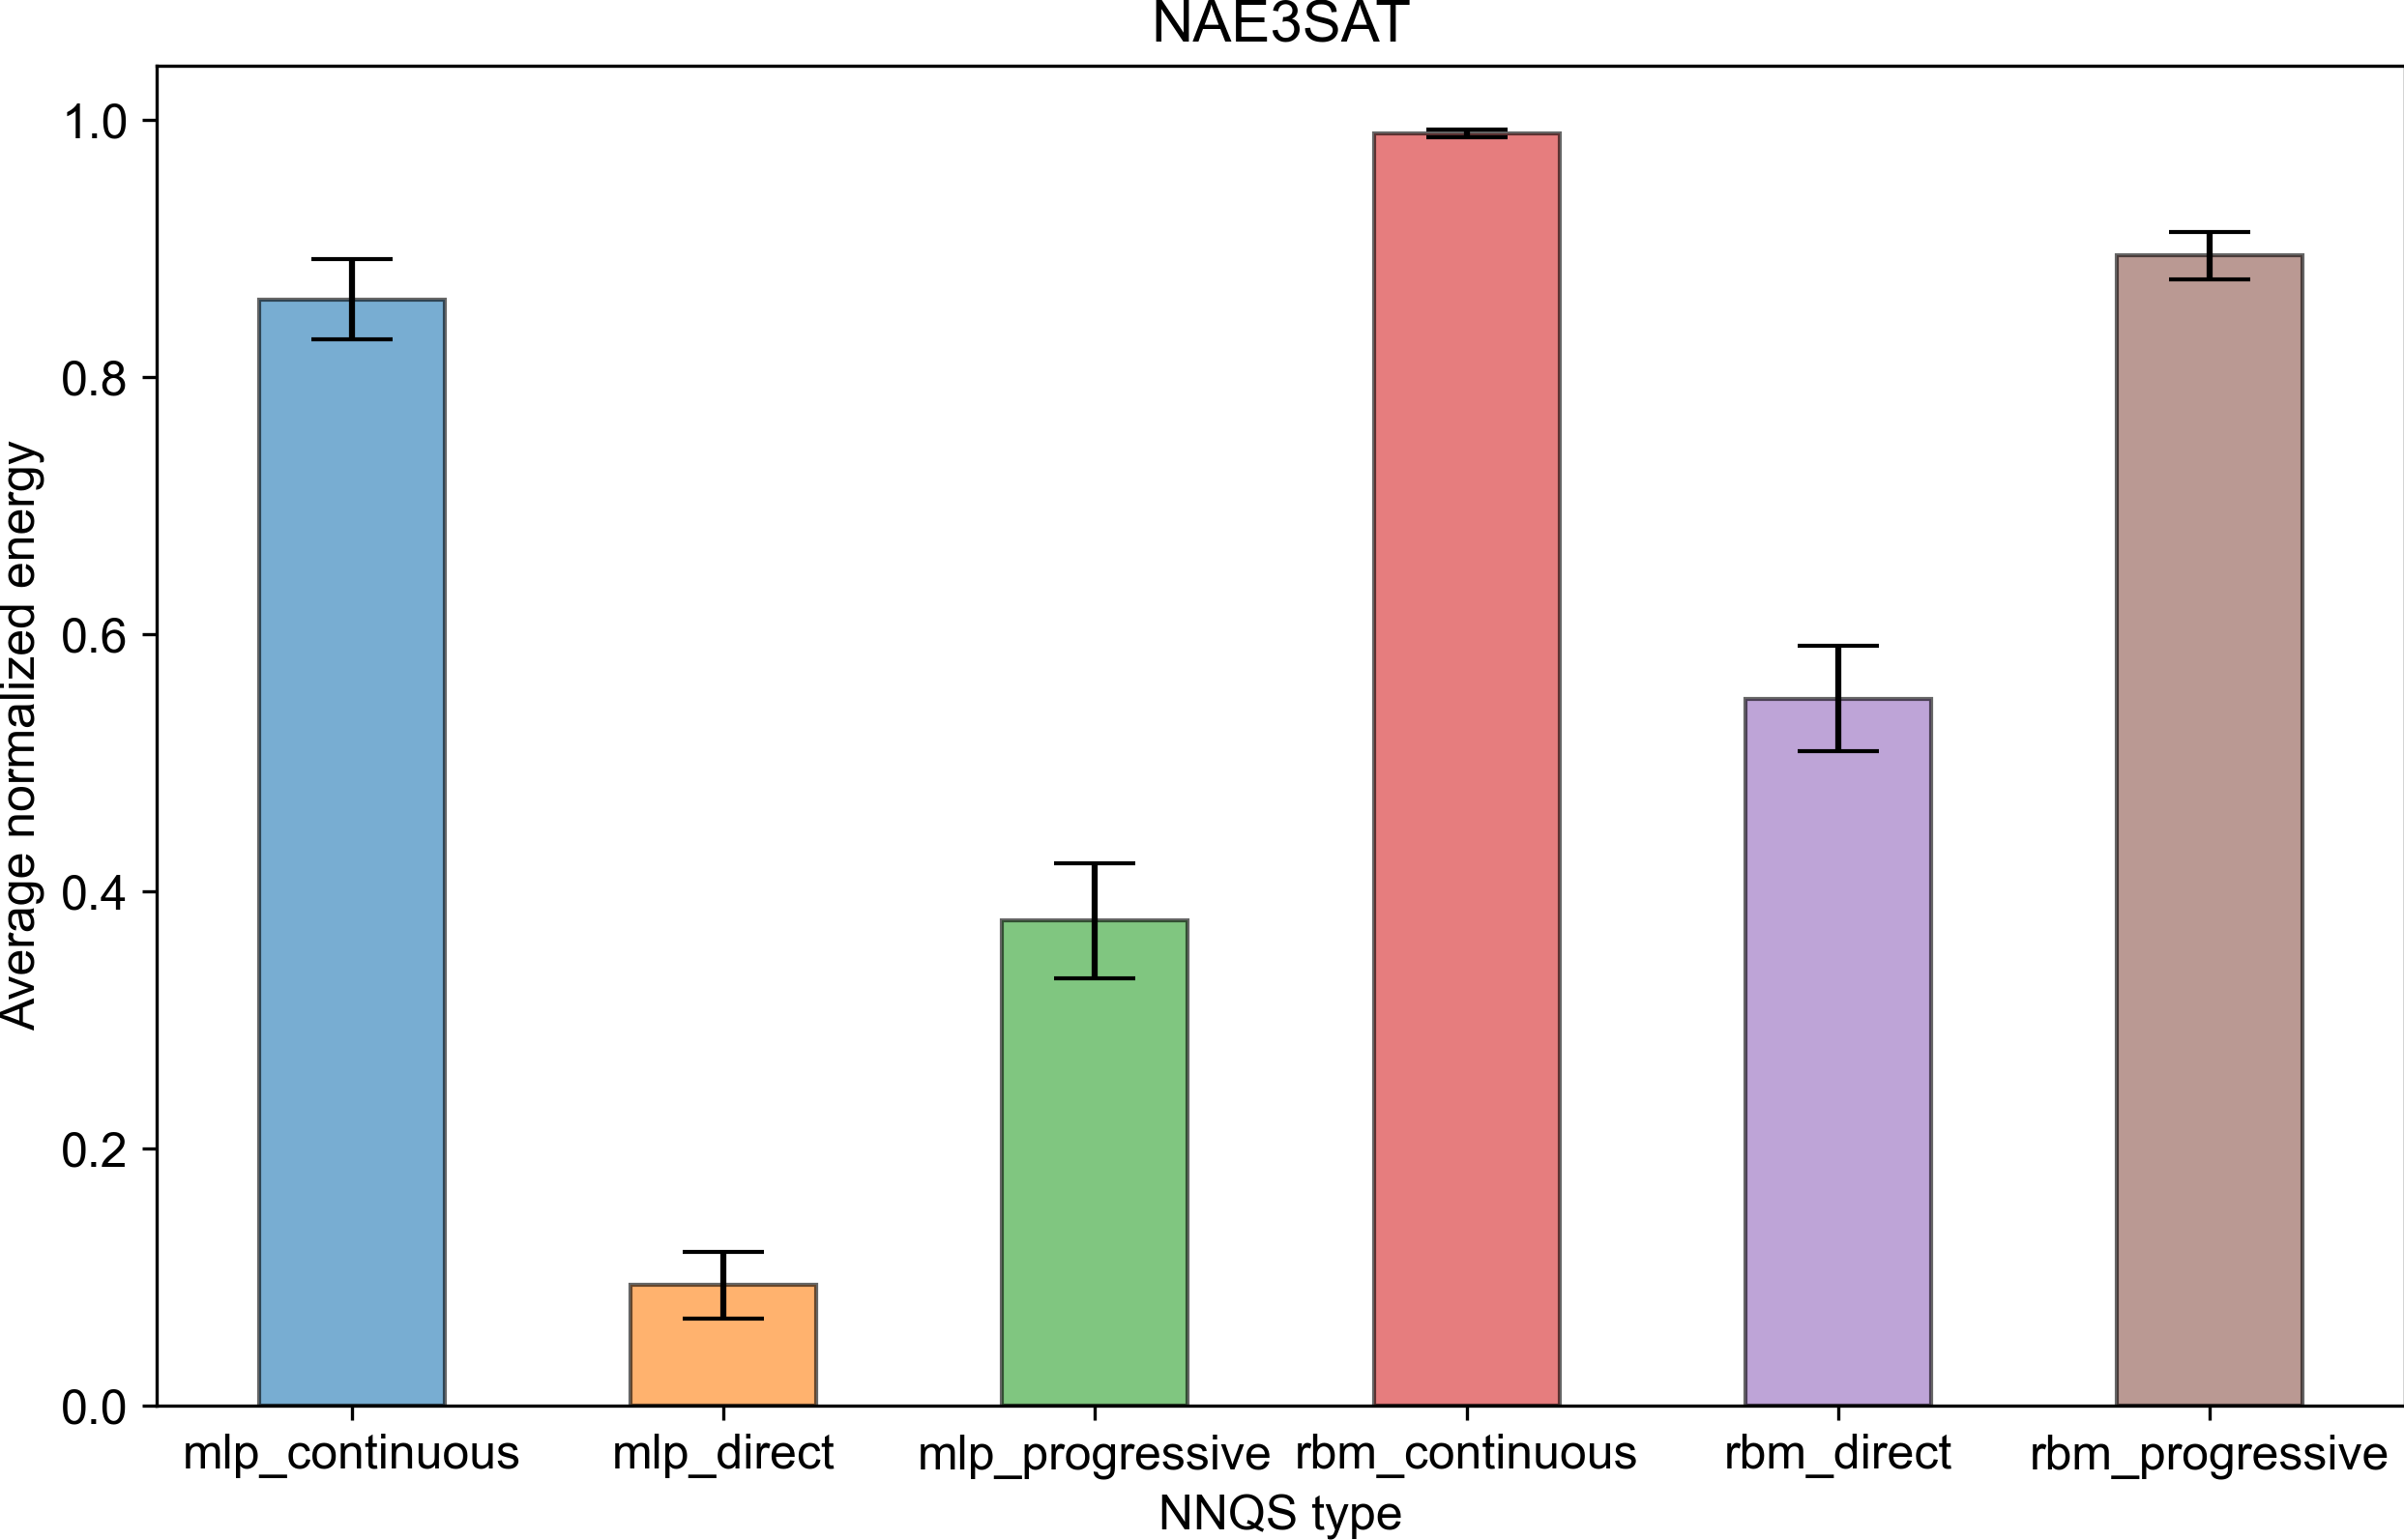
\includegraphics[width=0.5\textwidth]{images/nae3sat_nnqs_avg.png}}
    \subfloat[Success probability]{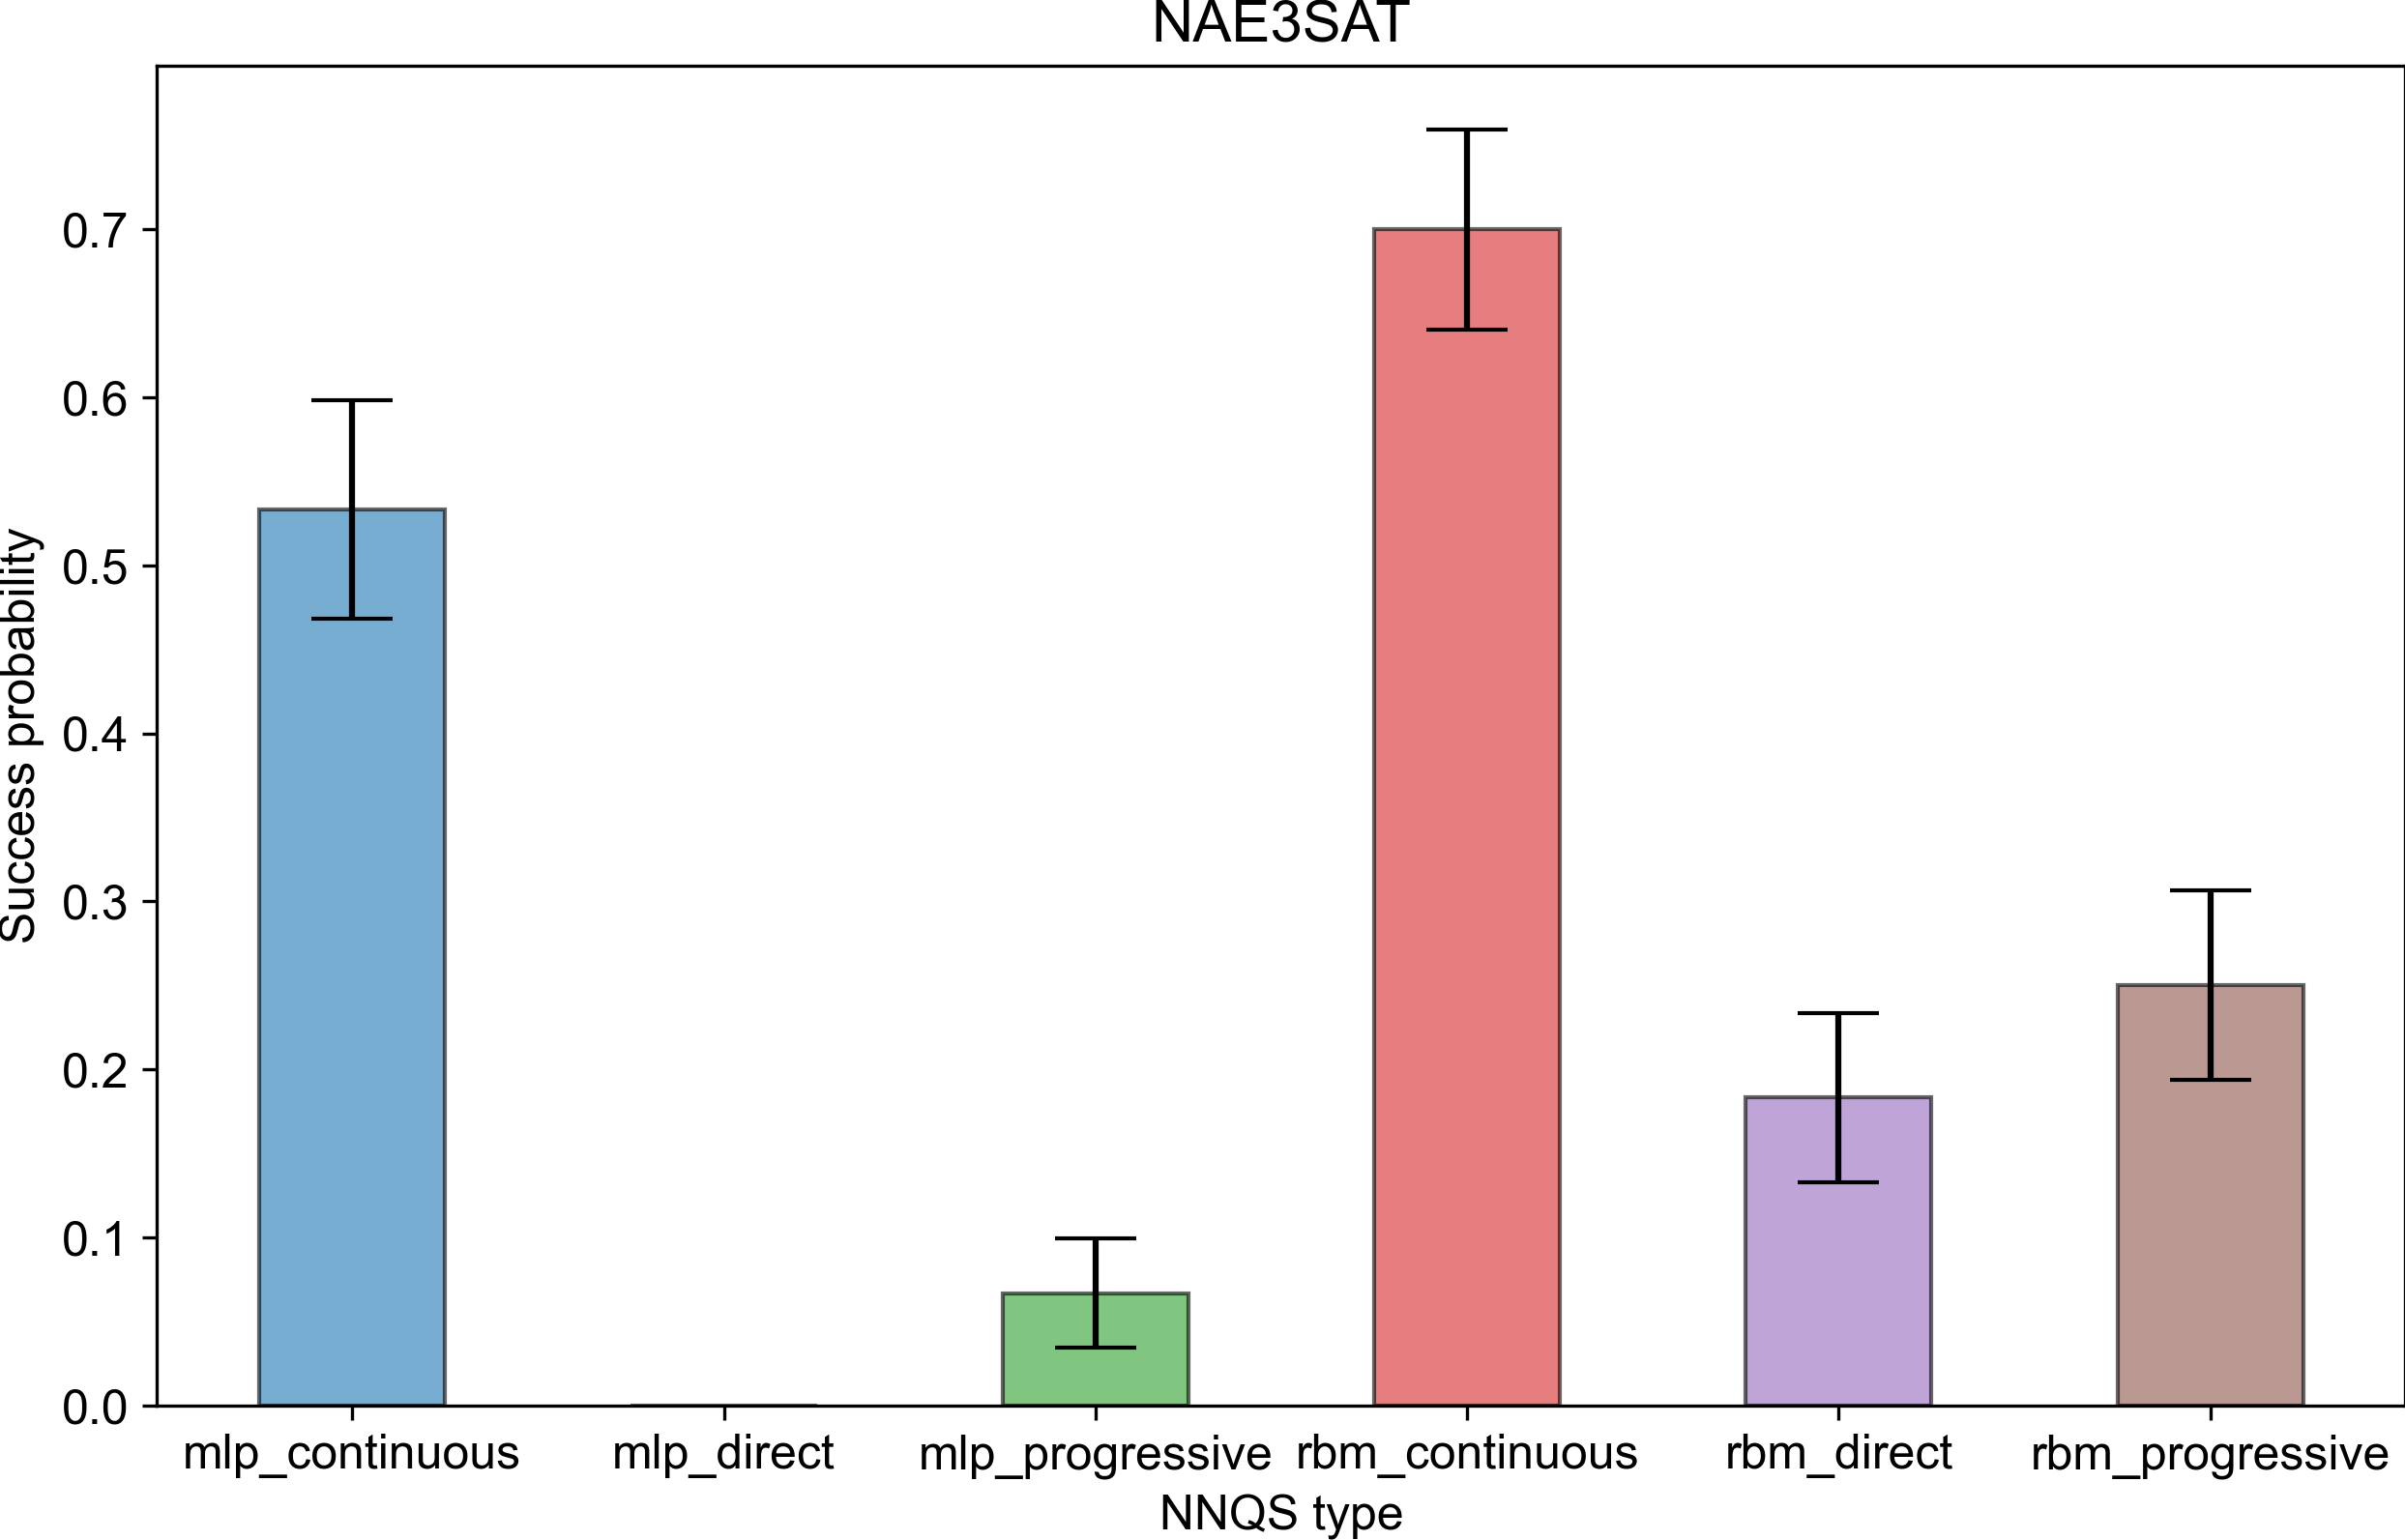
\includegraphics[width=0.5\textwidth]{images/nae3sat_nnqs_success_avg.png}}
    \caption{Average performance of different NNQS types for NAE3SAT}
    \label{nnqs-nae3sat-average}
\end{figure}

\subsection{Max-cut}
For the maxcut dataset, the RBM with continuous training (red) again performs the best in terms of average normalised energy and success probability when averaged across all sizes, shown in \autoref{nnqs-maxcut-average}. Again, the RBM with progressive training (brown), and the MLP with continuous training (blue) perform well. However, the performance gap between the top three solvers is relatively small, implying that max-cut might be easier than NAE3SAT.

\begin{figure}[!htb]
    \centering
    \subfloat[Normalised energy]{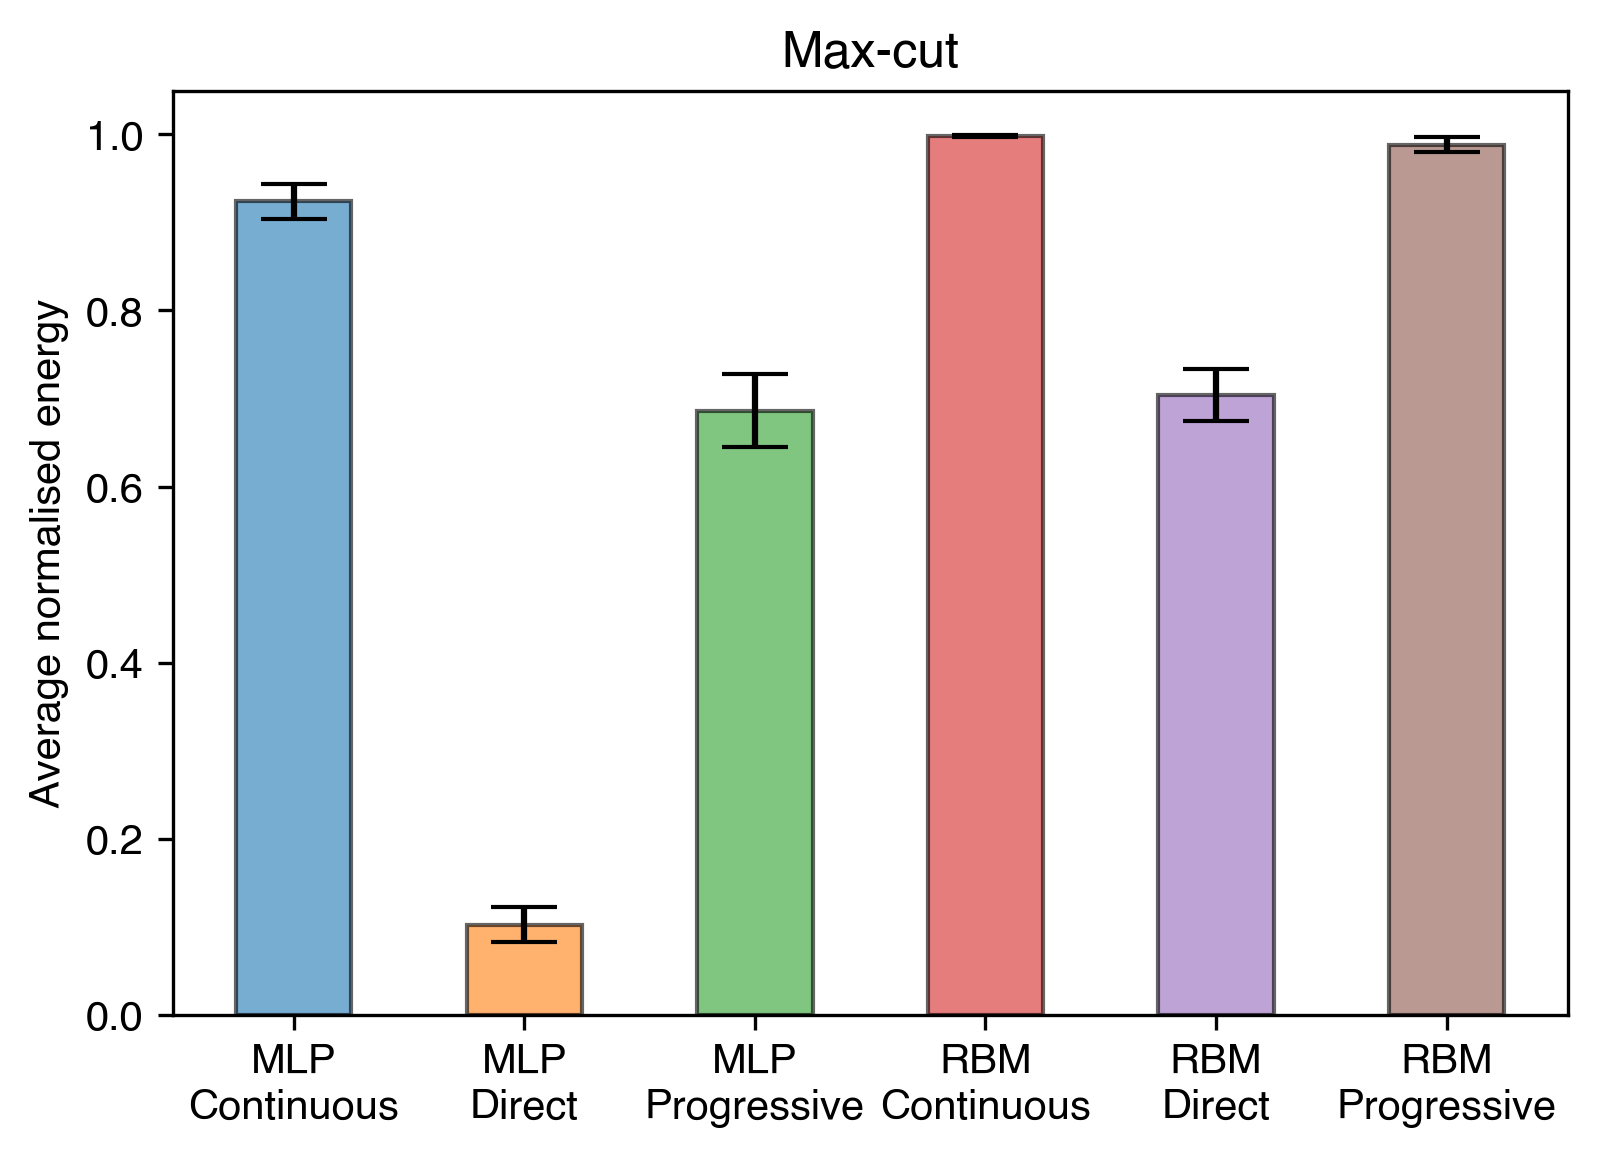
\includegraphics[width=0.5\textwidth]{images/maxcut_nnqs_avg.png}}
    \subfloat[Success probability]{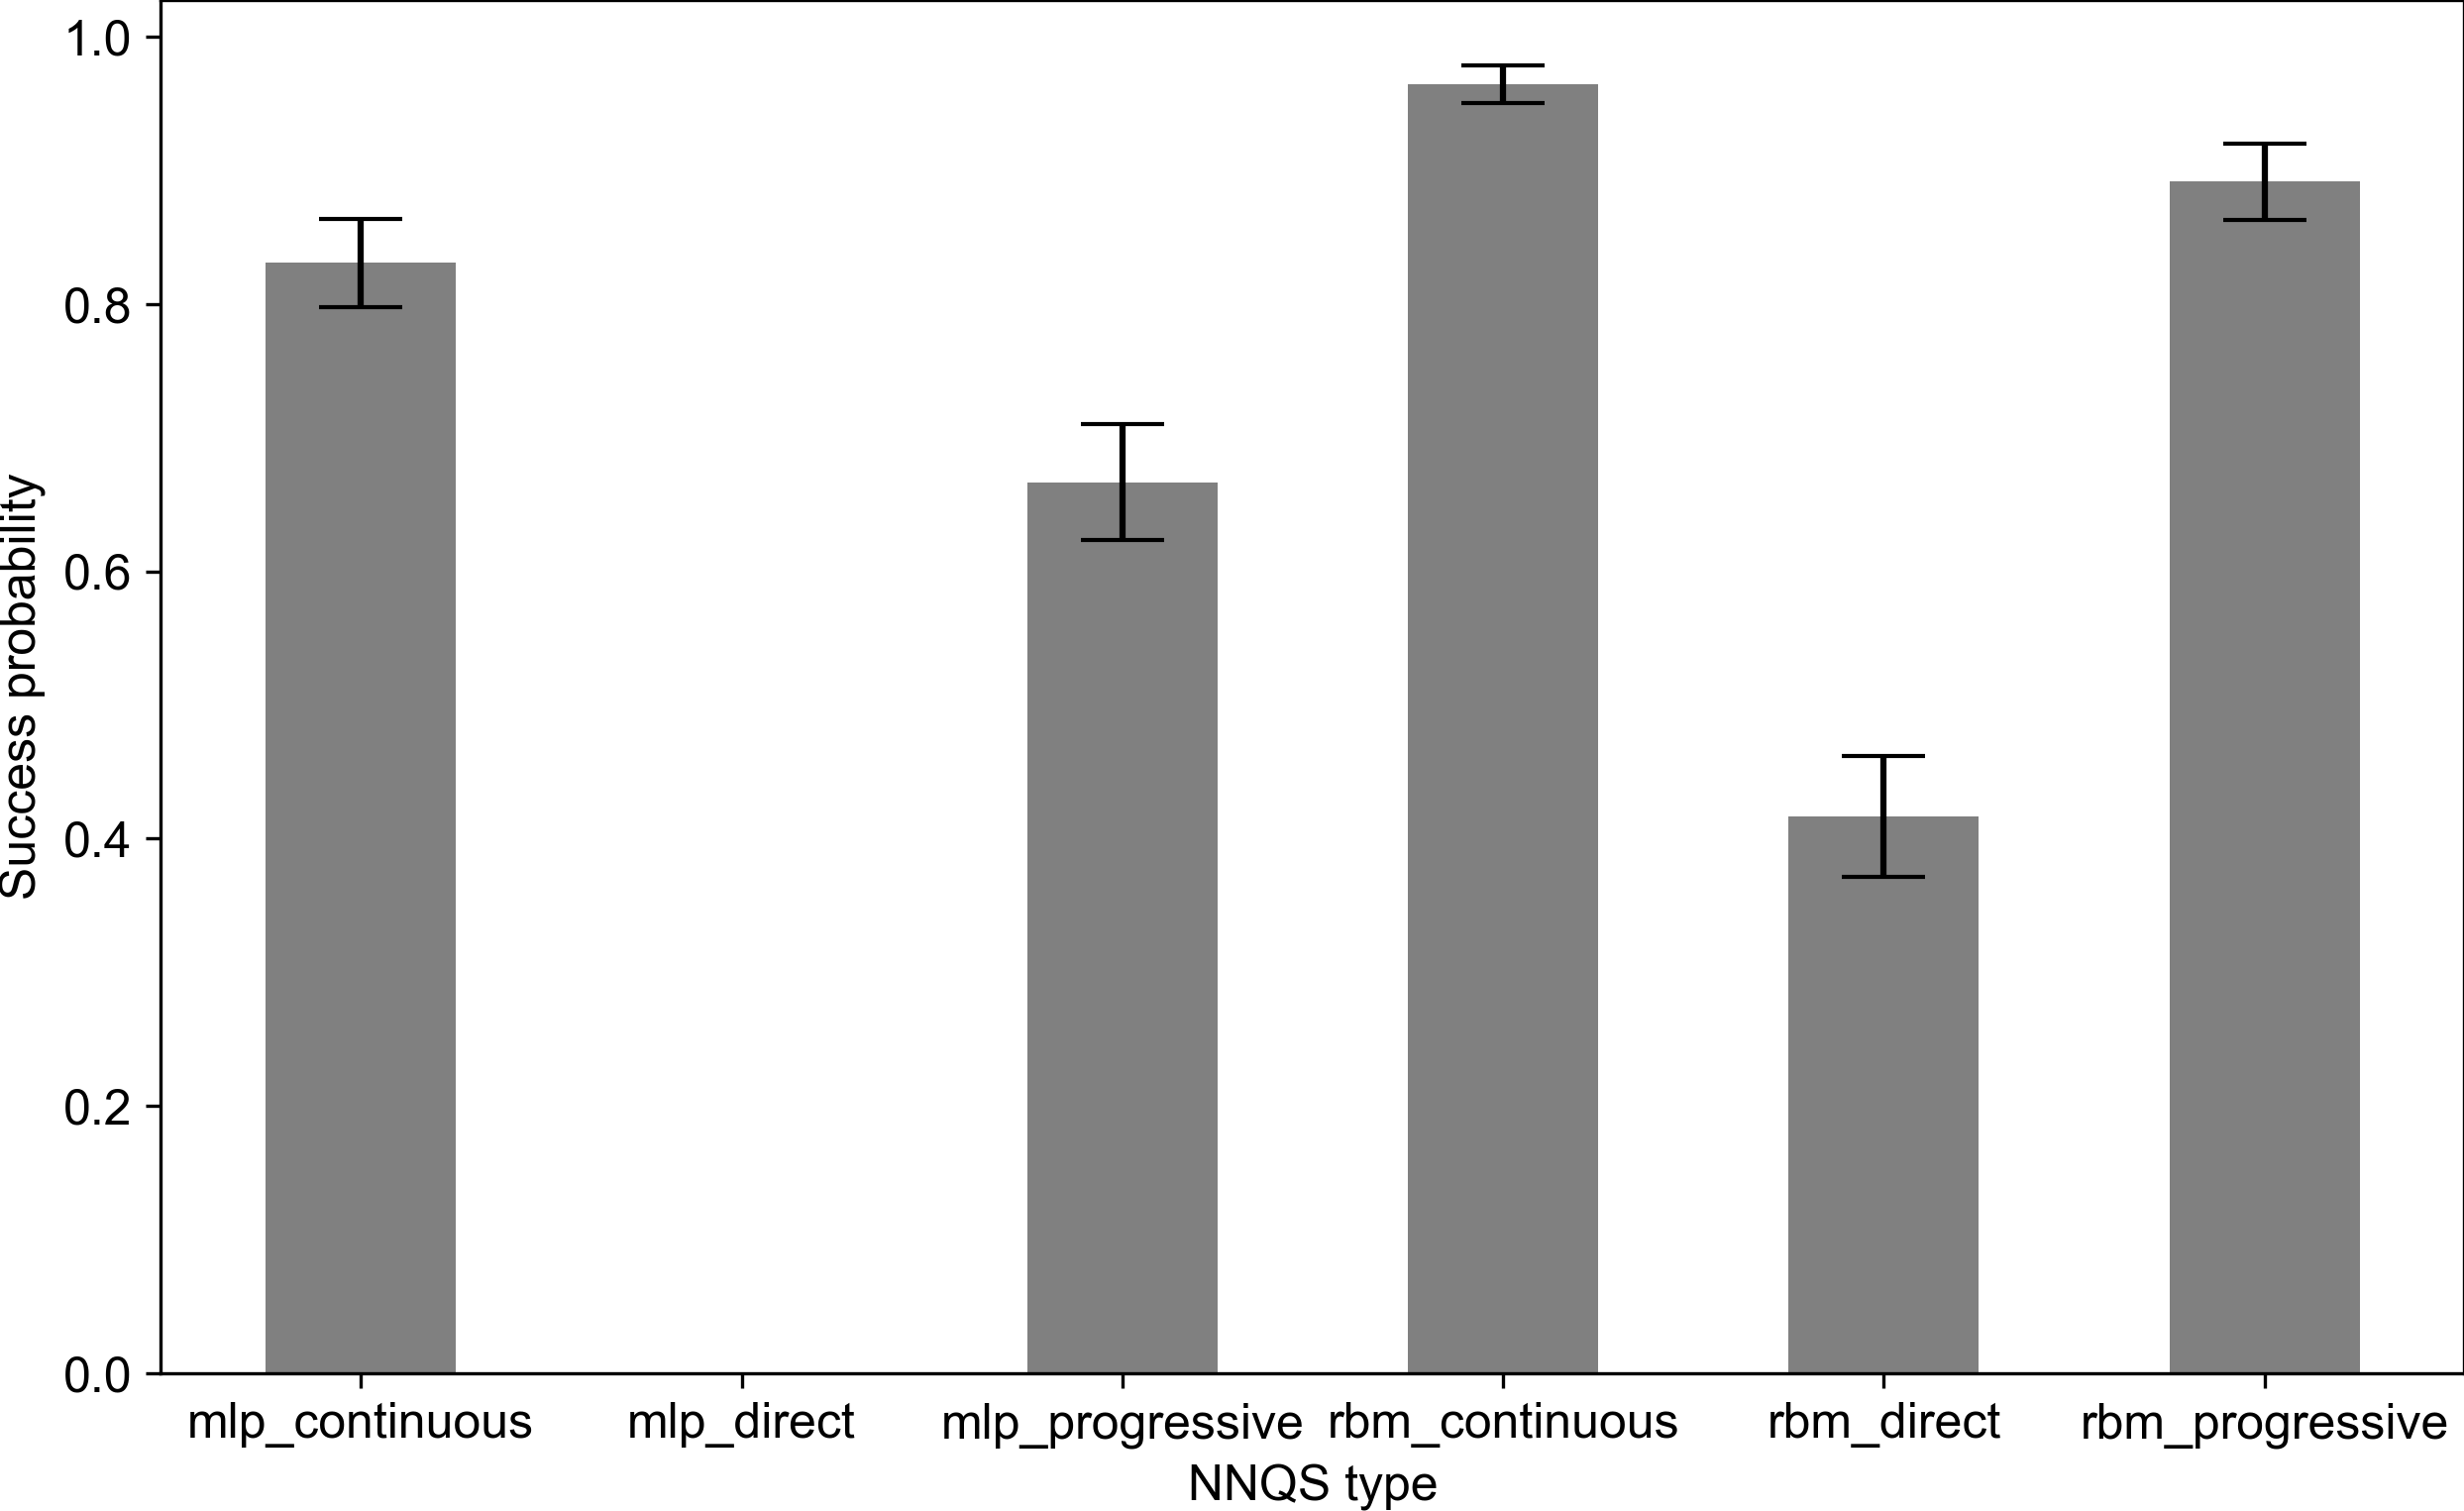
\includegraphics[width=0.5\textwidth]{images/maxcut_nnqs_success_avg.png}}
    \caption{Average performance of different NNQS types for max-cut}
    \label{nnqs-maxcut-average}
\end{figure}

\subsection{SK model}
For the SK model dataset, the RBM with continuous training (red) again performs the best in average normalised energy and success probability when averaged across all sizes, shown in \autoref{nnqs-skmodel-average}. The RBM with progressive training (brown) also perform well in both metrics.

\begin{figure}[!htb]
    \centering
    \subfloat[Normalised energy]{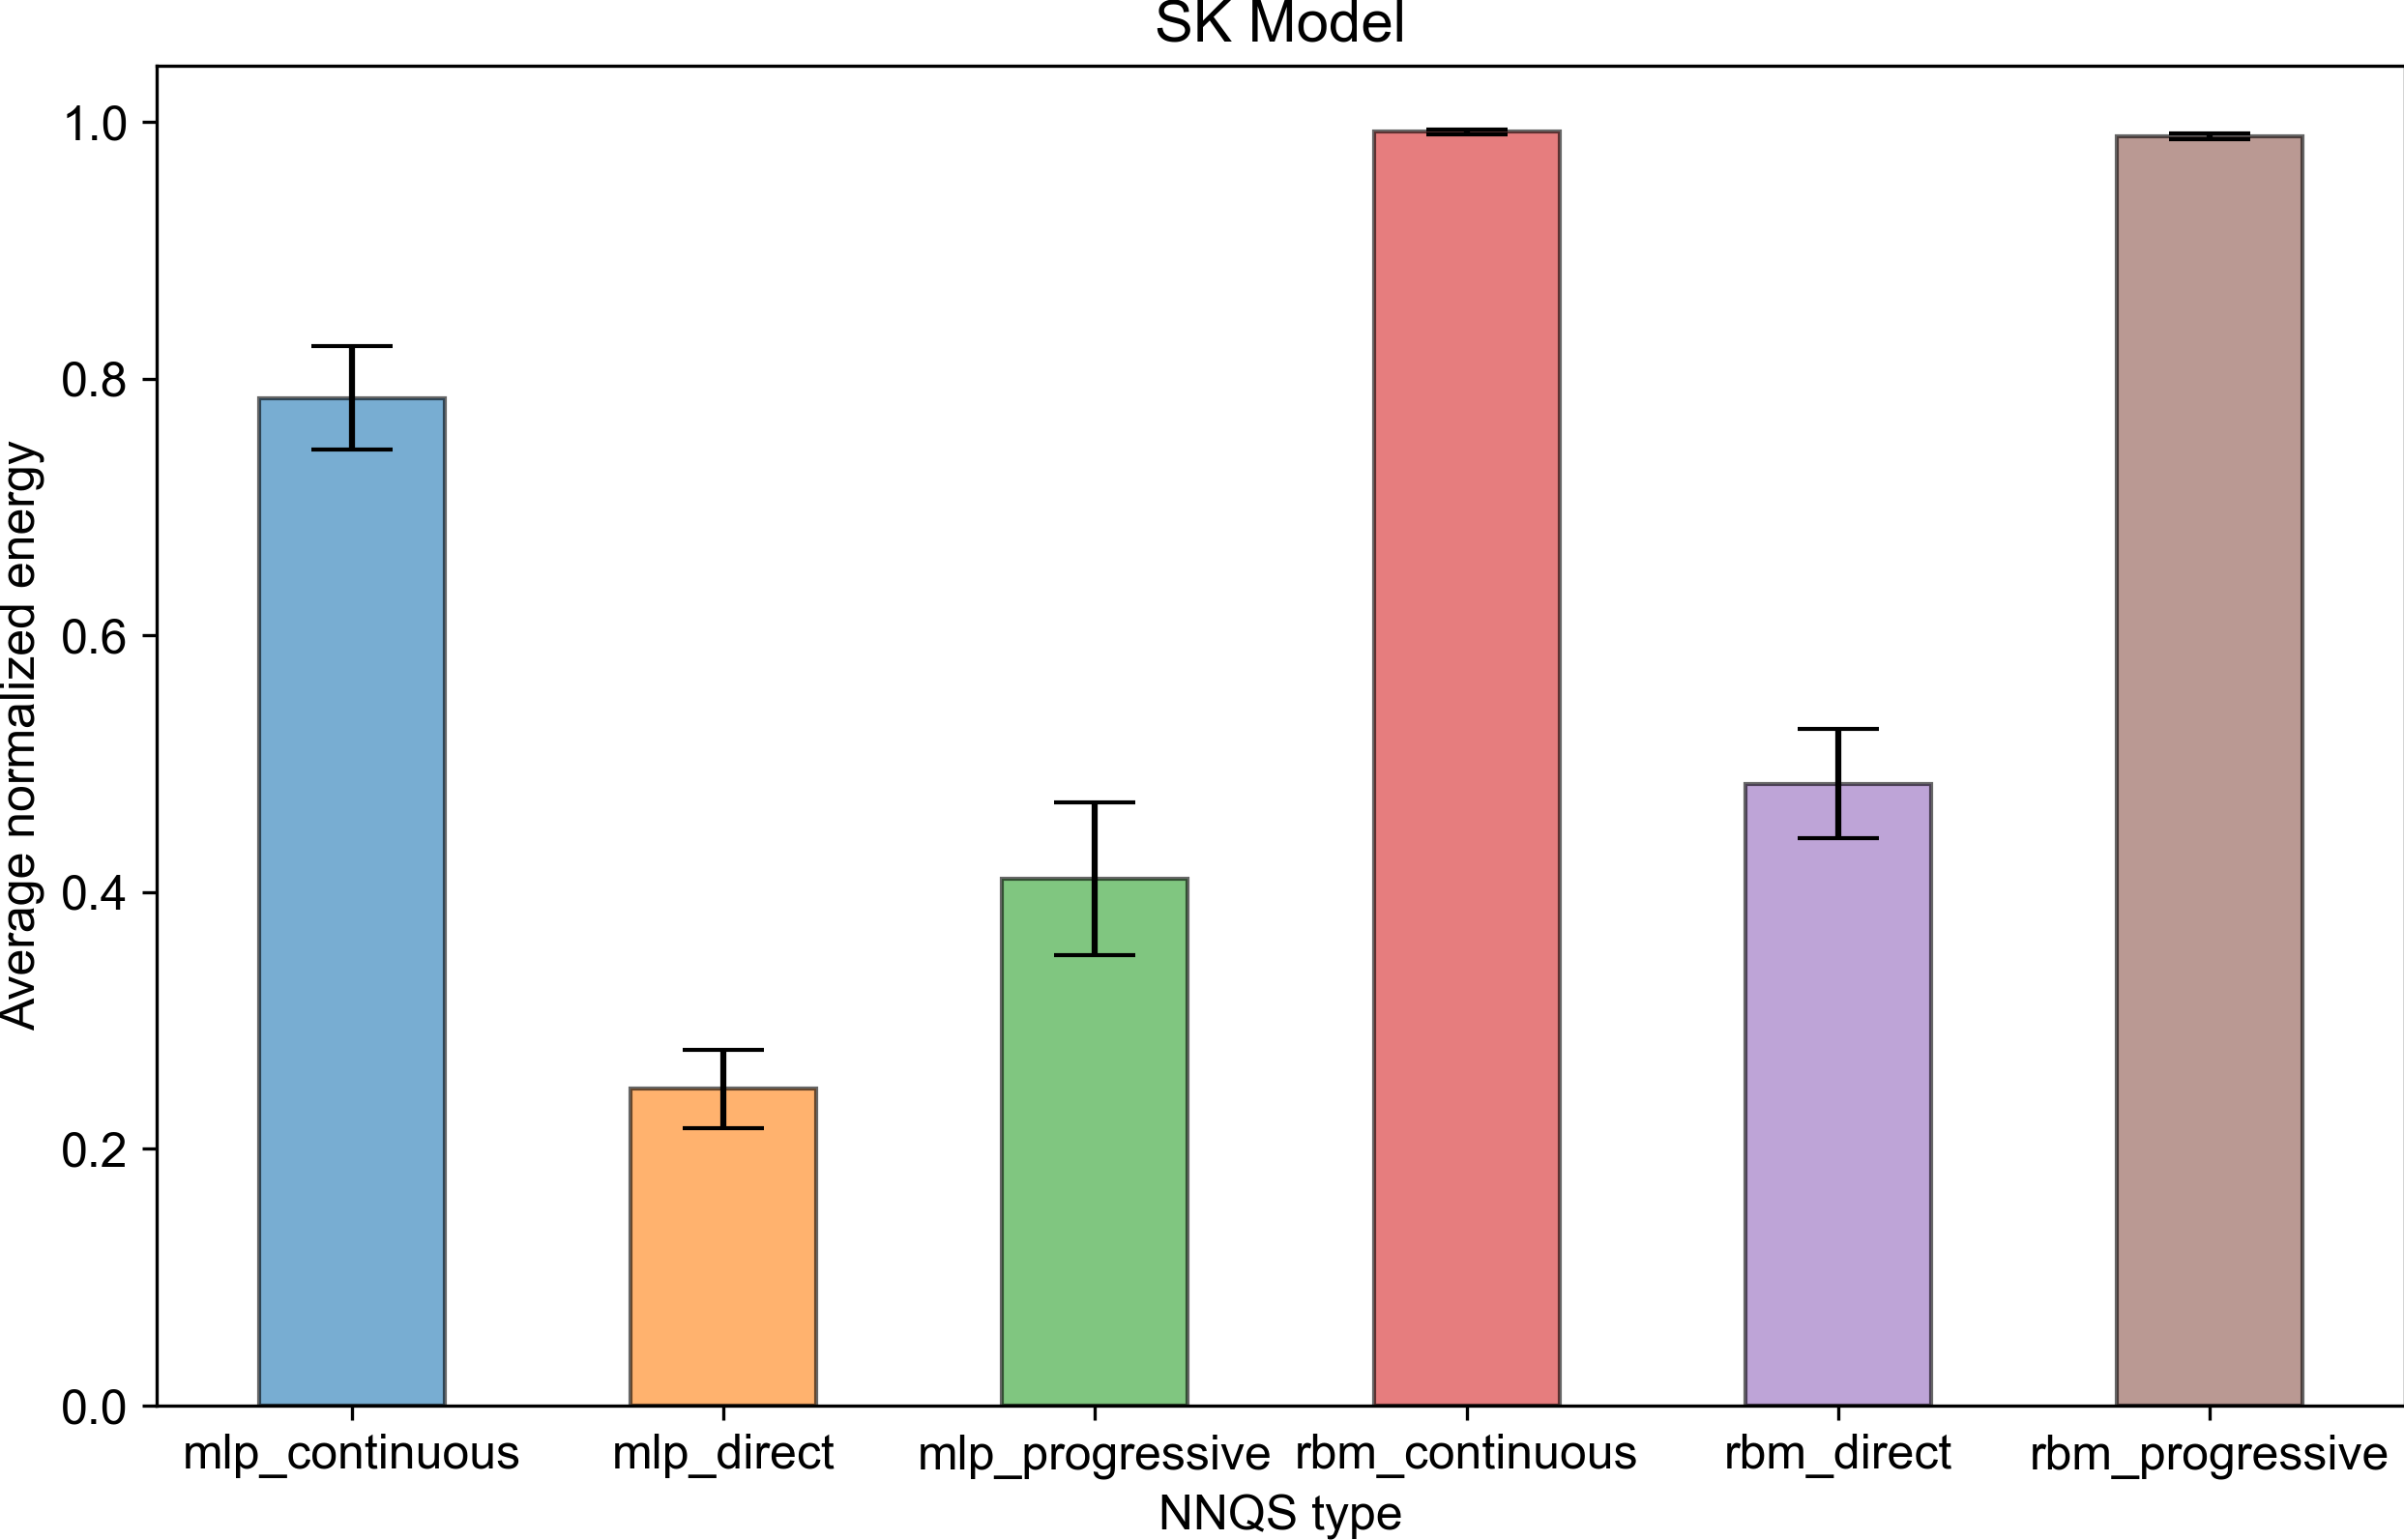
\includegraphics[width=0.5\textwidth]{images/skmodel_nnqs_avg.png}}
    \subfloat[Success probability]{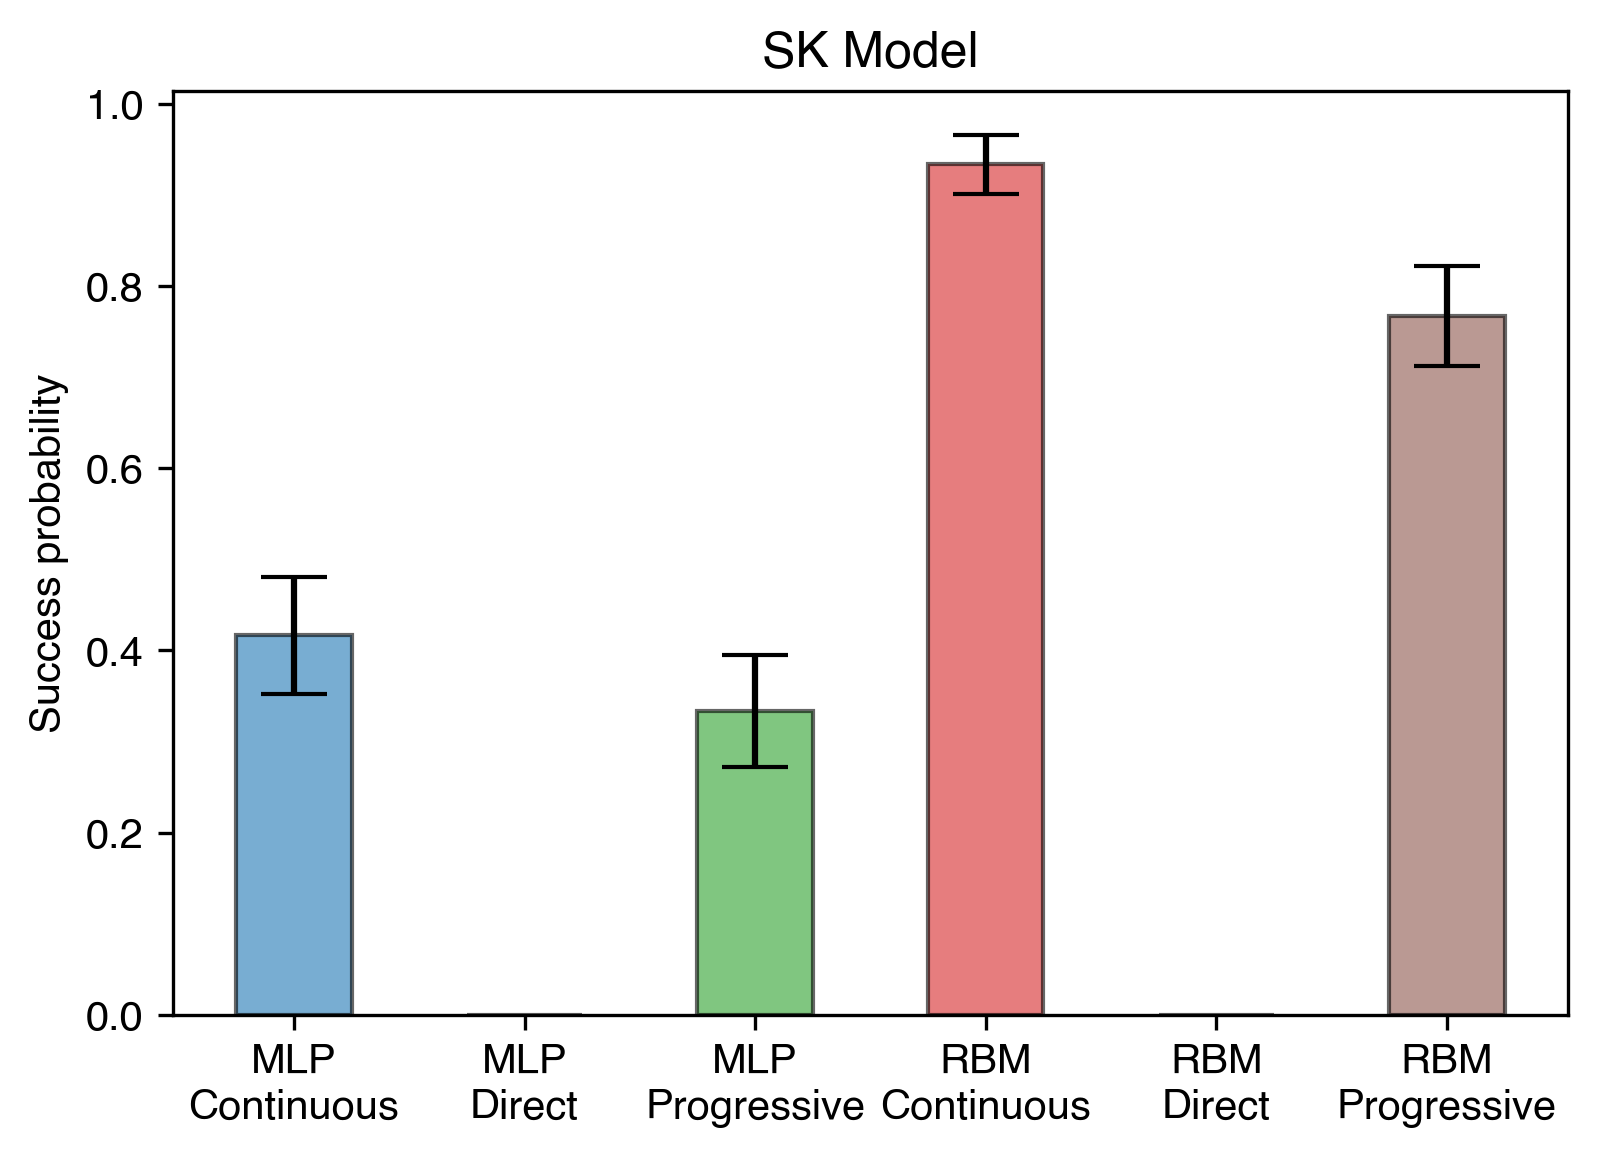
\includegraphics[width=0.5\textwidth]{images/skmodel_nnqs_success_avg.png}}
    \caption{Average performance of different NNQS types for SK model}
    \label{nnqs-skmodel-average}
\end{figure}

\section{Conclusion}
\autoref{results:nnqsnormalizedenergy} and \autoref{results:nnqssuccess} summarises the average normalised energy and success probability for different types of NNQS for each dataset and also computes the average across all datasets.

Comparing the two architectures, RBM performs better than MLP in both metrics for all datasets and training schemes. In terms of training schemes, direct training performs the worst among the three, and continuous training performs slightly better than progressive training. Using the RBM with a continuous training scheme gives the best performance across all datasets. 

The RBM likely performs better as it utilises Gibbs sampling, which is a more efficient sampling method and helps the neural network approximate the wave function more closely. Gibbs sampling allows for multiple-bit flips in each iteration and is thus able to explore a larger state space.

Even though progressive training more closely mimics the quantum annealing process in D-Wave solvers, the sudden change of Hamiltonian may have led to large gradient terms that made it more difficult for the neural network to converge, leading to poorer training. Continuous training gradually changes the Hamiltonian, which limits the gradient magnitudes and may result in better training. Even though continuous training performs better, we use progressive training in previous sections as our goal is to simulate the D-Wave annealing process and we do not fully understand why continuous training performs better. Direct training is expected to perform poorly as it tends to get stuck in local minima during training. 

\begin{table}[!htb]
    \centering
    \caption{Average normalised energy for different NNQS types}
    \label{results:nnqsnormalizedenergy}
    \begin{tabular}{ccccccc} \toprule
        ~ & \multicolumn{3}{c}{MLP} & \multicolumn{3}{c}{RBM} \\
        \cmidrule{2-7} & Continuous & Direct & Progressive & Continuous & Direct & Progressive \\
        \midrule
        NAE3SAT & 0.866 & 0.118 & 0.352 & \textbf{0.997} & 0.511 & 0.910 \\
        Max-cut & 0.924 & 0.102 & 0.686 & \textbf{0.998} & 0.704 & 0.988 \\
        SK model & 0.790 & 0.248 & 0.411 & \textbf{0.999} & 0.488 & 0.995 \\ \midrule
        Average & 0.860 & 0.156 & 0.483 & \textbf{0.998} & 0.568 & 0.965 \\ \bottomrule
    \end{tabular}
\end{table}

\begin{table}[!htb]
    \centering
    \caption{Success probability for different NNQS types}
    \label{results:nnqssuccess}
    \begin{tabular}{ccccccc} \toprule
        ~ & \multicolumn{3}{c}{MLP} & \multicolumn{3}{c}{RBM} \\
        \cmidrule{2-7} & Continuous & Direct & Progressive & Continuous & Direct & Progressive \\
        \midrule
        NAE3SAT & 0.583 & 0.029 & 0.062 & \textbf{0.950} & 0.167 & 0.364 \\
        Max-cut & 0.831 & 0.000 & 0.667 & \textbf{0.965} & 0.417 & 0.892 \\
        SK model & 0.417 & 0.000 & 0.333 & \textbf{0.933} & 0.000 & 0.767 \\ \midrule
        Average & 0.610 & 0.010 & 0.354 & \textbf{0.949} & 0.194 & 0.674 \\ \bottomrule
    \end{tabular}
\end{table}